%
\section{System overview}
\label{sec:system-overview}
The system overview presents a global view of the system, considering its main
features, components and interactions. It is not intended to be complete, but
rather provide a basis for the outline of the system architecture.
Fig.~\ref{fig:sys-overview} presents the \gls{mdo} system overview.
%
\begin{figure}[htb!]
\centering
    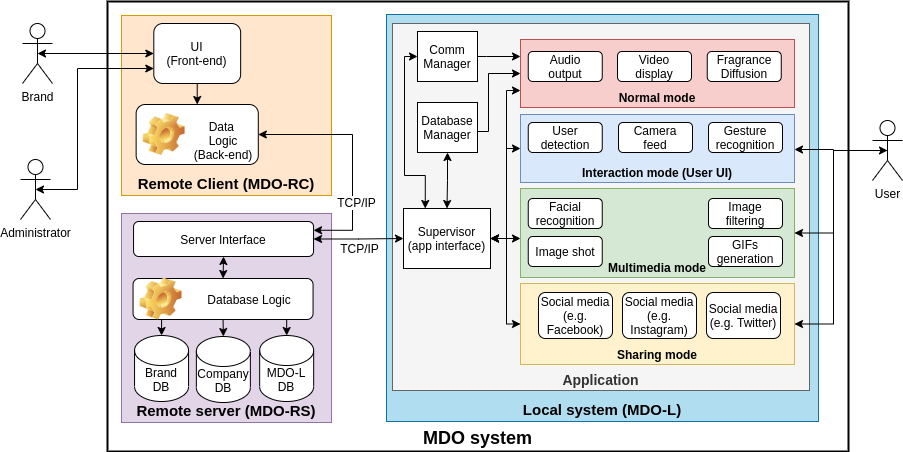
\includegraphics[width=1.0\columnwidth]{./img/sys-overview.png}
  \caption{\gls{mdo} system overview}%
\label{fig:sys-overview}
\end{figure}

Considering the system interactions, three main actors were identified:
\begin{enum-c}
\item \emph{Brand}: represents the brands contracting the advertisement
  services;
\item \emph{Company staff}: the development company staff, which can monitor and
  control the outdoor.
\item \emph{User}: the user (the target audience of the advertisiment)
  interacting with the system.
\end{enum-c}

Considering the data flow across the \textbf{MDO system}, three main subsystems were
identified: \textbf{\gls{mdo-rc}}, \textbf{\gls{mdo-rs}}, and
\textbf{\gls{mdo-l}}. The rational behind this initial decomposition is
explained next.

\subsection{MDO Remote Client}
The \emph{Brand} and \emph{Company Staff} members require a remote \gls{ui} (front-end) to
interact with the system: the former to configure the advertisements being
displayed at the \gls{mdo} and purchase them; the latter to remotely monitor and
control the operation of the \gls{mdo}. Thus, it is clear that \emph{an
  authentication mechanism must be provided for the remote \gls{ui}}.

The data is then dispatched to the back-end, where it is processed and feed back
to the \gls{ui} user and/or sent to the remote server, via \gls{tcp-ip}
comprising the data logic component of the \gls{ui}.
%
%
\subsection{MDO Remote Server}
\label{sec:mdo-remote-server}
Although the \gls{mdo-rc} could communicate directly with the \gls{mdo-l}, this
is not desirable or a good architecture mainly due to: communications failure could
result in data loss, compromising the system's integrity; the remote client and
the local system become tightly coupled, meaning the remote client must be aware
of all the available local systems; if the data storage in the local system
fails, the remote client would have to provide the backup information.

Thus, a remote server component is included, providing the access and management
of the system databases, pertaining to the \emph{Brand}, \emph{Company}, and
\emph{MDO Local system}. The first two provide the historical information of the
\texttt{Brand} and \texttt{Company} entities, and the last one the information
related to all of the \texttt{\gls{mdo-l}} systems in operation.

The main functions of the \texttt{\gls{mdo-rs}} are:
\begin{item-c}
\item \emph{UI requests responses}: when a \gls{ui} user requests/modifies
  some information from the database, the server must provide/update it.
\item \emph{\gls{mdo-l} monitoring and control}: provide command dispatch and
  feedback to the \texttt{Company} staff for remote monitoring and control of
  the device.
\item \emph{\gls{mdo-l} update}: periodically check for start times of each
  \gls{mdo-l} device and transfer the relevant data to it.
\end{item-c}
%

\subsection{MDO Local system}
\label{sec:mdo-local-system}




%%% Local Variables:
%%% mode: latex
%%% TeX-master: "../../../dissertation"
%%% End:
